\documentclass[journal]{IEEEtran}
\usepackage{amsmath,amsfonts}
\usepackage{algorithmic}
\usepackage{algorithm}
\usepackage{amssymb}
\usepackage{array}
\usepackage[caption=false,font=normalsize,labelfont=sf,textfont=sf]{subfig}
\usepackage{textcomp}
\usepackage{stfloats}
\usepackage{url}
\usepackage{verbatim}
\usepackage{graphicx}
\usepackage{cite}
\usepackage{xcolor}
\hyphenation{op-tical net-works semi-conduc-tor IEEE-Xplore}
\usepackage{hyperref}
\hypersetup{
  colorlinks=true,   % Enable colored links
  linkcolor=blue,    % Set internal links to blue
  citecolor=blue,    % Set citation links to blue
  urlcolor=blue      % Set URL links to blue
}
\usepackage{booktabs} % for \hline
\renewcommand{\algorithmicrequire}{\textbf{Input:}}
\renewcommand{\algorithmicensure}{\textbf{Output:}}
\usepackage{threeparttable}
\usepackage{amsthm}
\newtheorem{definition}{Definition}
\newtheorem{proposition}{Proposition}
\usepackage{listings}
\usepackage{tikz}
\usetikzlibrary{shapes,arrows,positioning,calc,shadows}

\begin{document}

\title{Optimized Parallel Architectures of Post-Quantum Signature SPHINCS\textsuperscript{+} on GPUs}

\author{Jiahao Xiang and Lang Li.

  \thanks{This work is supported by the Hunan Provincial Natural Science Foundation of China (2022JJ30103), Postgraduate Scientific Research Innovation Project of Hunan Province (CX20240977), “the 14th Five-Year Plan” Key Disciplines and Application-oriented Special Disciplines of Hunan Province (Xiangjiaotong [2022] 351), the Science and Technology Innovation Program of Hunan Province (2016TP1020).}

  \thanks{Jiahao Xiang and Lang Li are affiliated with the Hunan Provincial Key Laboratory of Intelligent Information Processing and Application, as well as the Hunan Engineering Research Center of Cyberspace Security Technology and Applications, both located at Hengyang Normal University, Hengyang 421002, China. They are also faculty members of the College of Computer Science and Technology at Hengyang Normal University. (e-mail: jiahaoxiang2000@gmail.com; lilang911@126.com)}% <-this % stops a space
}
% \thanks{Manuscript received April 19, 2021; revised August 16, 2021.}}
% \thanks{Manuscript received }}

% The paper headers
\markboth{Journal of \LaTeX\ Class Files,~Vol.~14, No.~8, August~2021}%
{Shell \MakeLowercase{\textit{et al.}}: A Sample Article Using IEEEtran.cls for IEEE Journals}

\IEEEpubid{}
% Remember, if you use this you must call \IEEEpubidadjcol in the second
% column for its text to clear the IEEEpubid mark.

\maketitle

\begin{abstract}

  The Post-Quantum Cryptography (PQC) standardization process has led to the development of SPHINCS\textsuperscript{+}, a stateless hash-based signature scheme that provides long-term security. The high computational cost of SPHINCS\textsuperscript{+} has motivated research into efficient implementations on various platforms. In this work, we present a GPU-based implementation of SPHINCS\textsuperscript{+} that achieves high throughput while maintaining security guarantees. Our implementation leverages the parallel processing capabilities of GPUs to accelerate the signature generation process. We evaluate the performance of our implementation on an NVIDIA RTX 4090 GPU and demonstrate that it can achieve a throughput of xxx for the SPHINCS\textsuperscript{+} signature generation. Our results show that GPUs can be an effective platform for accelerating SPHINCS\textsuperscript{+} and other post-quantum cryptographic schemes.

\end{abstract}

\begin{IEEEkeywords}
  Software implementation, GPU, signature algorithm.
\end{IEEEkeywords}

\section{Introduction}
\label{sec:intro}

\IEEEPARstart{T}{he} quantum computers leverage quantum-mechanical phenomena to process data, raising significant concerns about the resilience of classical cryptographic methods.
The security offered by widely deployed public-key cryptosystems, such as RSA and ECC, is jeopardized by Shor's algorithm \cite{Shor1994}, motivating comprehensive research on alternative cryptographic solutions. In response, the National Institute of Standards and Technology (NIST) initiated the Post-Quantum Cryptography (PQC) standardization process to develop novel schemes that withstand quantum computing capabilities \cite{NIST2016}.

SPHINCS\textsuperscript{+} is a representative stateless hash-based signature scheme and a finalist in the ongoing NIST standardization effort \cite{Turan}. Long-term security against advanced quantum attacks is targeted by employing robust cryptographic hash functions \cite{Bernstein2019}. The high computational cost of SPHINCS\textsuperscript{+} has motivated further investigations into efficient implementations across CPUs, FPGAs, and GPUs \cite{Joseph2022} to facilitate smooth adoption by organizations transitioning to post-quantum cryptography.

\subsection{Related Work}

Recent years have witnessed significant progress in GPU-based implementations of SPHINCS\textsuperscript{+}. Lee and Hwang~\cite{Lee2022} pioneered the exploration of GPU acceleration for post-quantum cryptographic schemes, establishing foundational techniques for parallel implementation of hash-based signatures. Building upon this foundation, Kim et al.~\cite{Kim2024} introduced parallel methods for key components of SPHINCS\textsuperscript{+}, including FORS, WOTS\textsuperscript{+}, and MSS tree computations. Their implementation on an RTX 3090 GPU demonstrated significant throughput improvements, though it faced efficiency limitations due to multiple CUDA kernel launches.

Most recently, Wang et al.~\cite{Wang2025} presented CUSPX, introducing a comprehensive three-level parallelism framework that integrates algorithmic, data, and hybrid parallelization strategies. Their implementation incorporated novel parallel Merkle tree construction algorithms and multiple load-balancing approaches, achieving substantial performance improvements over previous implementations. Additionally, Ning et al.~\cite{Ning2024} proposed GRASP, which further optimized GPU-based SPHINCS\textsuperscript{+} implementation through adaptive parallelization strategies and kernel fusion technology.

\subsection{Motivation}

While previous implementations have made significant strides in GPU acceleration of SPHINCS\textsuperscript{+}, several critical aspects remain unexplored. Existing approaches primarily focus on maximizing throughput through extensive parallelization, often overlooking the efficiency of individual thread execution. The implementation by Kim et al.~\cite{Kim2024} demonstrated the potential of parallel processing but was limited by multiple kernel launches. Although CUSPX~\cite{Wang2025} introduced a comprehensive parallelization framework, its approach to thread utilization could be further optimized.

Two key observations motivate our work. First, current implementations typically concentrate on parallelizing the SPHINCS\textsuperscript{+} algorithm structure while paying less attention to the parallel optimization of underlying hash functions. A more holistic approach that considers both algorithmic levels could yield better performance. Second, existing implementations often prioritize maximum parallelism without fully considering the trade-off between thread count and execution efficiency. This can lead to suboptimal performance due to increased synchronization overhead and reduced work efficiency per thread.

These observations suggest the need for a more balanced approach that optimizes both the degree of parallelism and the computational efficiency of individual threads. Our work aims to address these limitations by developing an implementation that not only leverages GPU parallelism effectively but also ensures efficient utilization of computational resources at the thread level.

\subsection{Contributions}

In this brief, an optimized GPU-based implementation of SPHINCS\textsuperscript{+} is presented, achieving high throughput without compromising security. The main contributions are summarized as follows:

\begin{enumerate}
  \item A novel parallelization strategy is introduced that balances the degree of parallelism with the computational efficiency of individual threads, thereby enhancing GPU resource utilization.
  \item The parallel architectures of SPHINCS\textsuperscript{+} are optimized by integrating algorithmic and data-level parallelization techniques, which improve the performance of the underlying hash functions.
  \item The implementation is evaluated on an NVIDIA GPU, demonstrating a throughput of XXX SPHINCS\textsuperscript{+} signatures per second, significantly exceeding the performance of state-of-the-art approaches. The complete source code and implementation details are available at \url{https://github.com/jiahaoxiang2000/sphincs-plus}.
\end{enumerate}
The remainder of the brief is organized as follows. Section~\ref{sec:preliminaries} provides an overview of the SPHINCS\textsuperscript{+} signature scheme; Section~\ref{sec:implementation} details the GPU-based implementation; Section~\ref{sec:evaluation} presents the performance evaluation; and Section~\ref{sec:conclusion} concludes the brief.

\color{blue}

%% filepath: /Users/xiangjiahao/tex/ThirdPaper/tex/index.tex
% ...existing code...

\section{Preliminaries}\label{sec:preliminaries}

Essential background information on SPHINCS\textsuperscript{+} and GPU computing is provided in this section, forming the basis for the optimized implementation. First, the core components and security features of SPHINCS\textsuperscript{+} are discussed, including its hash-based signature structure and hierarchical certification tree. Then, the CUDA programming model and its parallel execution paradigm are explained, highlighting the relevance to GPU-based optimization.

\subsection{\texorpdfstring{SPHINCS\textsuperscript{+}}{SPHINCS+} Overview}

SPHINCS\textsuperscript{+} is a stateless hash-based signature scheme that delivers post-quantum security through a hierarchical certification structure. The signature generation process relies on three main components:

\begin{itemize}
  \item \textbf{WOTS+ (Winternitz One-Time Signature)}: A one-time scheme that handles authentication paths and underpins the Merkle tree construction
  \item \textbf{FORS (Forest Of Random Subsets)}: A few-time signature scheme that uses $k$ components, each containing $t$ elements selected from pseudorandom subsets
  \item \textbf{Hypertree}: A multi-layer structure of height $h$ divided into $d$ layers, each containing Merkle trees of height $h/d$ for authenticating WOTS+ public keys
\end{itemize}

\begin{figure}[t]
  \centering
  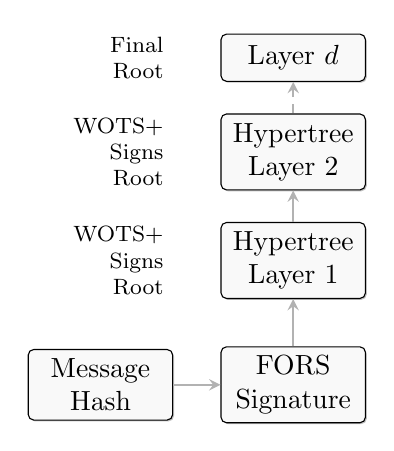
\begin{tikzpicture}[
      block/.style={
        rectangle,
        draw,
        fill=white,
        text width=1.6cm,
        align=center,
        minimum height=0.6cm,
        rounded corners=2pt,
        fill=gray!5,
        drop shadow={shadow xshift=0.5pt, shadow yshift=-0.5pt}
      },
      arrow/.style={->,>=stealth,thick,draw=gray!60},
      level/.style={sibling distance=35mm,level distance=0.7cm}
    ]
    % Message and Components
    \node[block] (fors) at (0,0) {FORS\\Signature};
    \node[block,left=0.6cm of fors] (hash) {Message\\Hash};

    % Hypertree Layers
    \node[block,above=0.6cm of fors] (ht1) {Hypertree\\Layer 1};
    \node[block,above=0.4cm of ht1] (ht2) {Hypertree\\Layer 2};
    \node[block,above=0.4cm of ht2] (htd) {Layer $d$};

    \draw[arrow] (hash) to (fors);
    \draw[arrow] (fors) to (ht1);
    \draw[arrow] (ht1) to (ht2);
    \draw[arrow] ($(htd)+(0,-0.5)$) -- (htd);
    \draw[dashed,thick,gray!60] ($(ht2)+(0,0.5)$) -- ($(htd)+(0,-0.3)$);

    \node[left=0.6cm of ht1,text width=1.4cm,font=\footnotesize,align=right] {WOTS+ Signs Root};
    \node[left=0.6cm of ht2,text width=1.4cm,font=\footnotesize,align=right] {WOTS+ Signs Root};
    \node[left=0.6cm of htd,text width=1.4cm,font=\footnotesize,align=right] {Final Root};
  \end{tikzpicture}
  \caption{SPHINCS\textsuperscript{+} signature generation flow. A message hash is signed by FORS to produce $k$ authentication paths, which are then authenticated by a $d$-layer hypertree. Each layer employs WOTS+ to sign the root of the previous layer, culminating in a final root signature.}
  \label{fig:sphincs-process}
\end{figure}

The SPHINCS\textsuperscript{+} signature generation process, shown in Figure~\ref{fig:sphincs-process}, employs a hierarchical authentication structure. A message digest is first created via hashing, followed by signing with the FORS few-time scheme, producing $k$ authentication paths of $t$ elements each. The resulting FORS public key is authenticated through a hypertree of $d$ layers, where each layer uses WOTS+ to sign the root of the layer below. This chain of signatures leads to the final root node, offering efficient verification with robust hash-based security.

Two operational modes, “simple” and “robust,” are provided to balance speed and security. Parameter sets facilitate trade-offs among signature size, security level, and computational efficiency. All security properties derive from the hash functions, rendering SPHINCS\textsuperscript{+} resistant to quantum attacks.

\subsection{GPU Computing Model}

Modern Graphics Processing Units (GPUs) incorporate a large number of cores organized within multiple Streaming Multiprocessors (SMs). This highly parallel structure supports Single Instruction, Multiple Thread (SIMT) execution, wherein threads are grouped into warps, and warps collectively form blocks. Each block is then scheduled across available SMs, ensuring that thousands of concurrent threads can execute similar instructions in parallel.

GPU architectures integrate various on-chip memories, including shared memory, registers, and caches, to enable efficient data exchange among threads within a block. These hardware components mitigate the bandwidth limitations associated with frequent global memory accesses. Consequently, GPU performance gains are visible when computational tasks exhibit substantial parallelism, as is the case in large-scale cryptographic algorithms such as SPHINCS\textsuperscript{+}.

In the CUDA framework, memory optimization strategies such as coalesced accesses, shared memory buffering, and constant memory utilization further enhance throughput. Extensive parallelization of SPHINCS\textsuperscript{+} computations is therefore facilitated, allowing performance improvements through a combination of thread-level, data-level, and algorithmic parallelism.

\color{black}

\section{Optimized Implementation of \texorpdfstring{SPHINCS\textsuperscript{+}}{SPHINCS+}}\label{sec:implementation}

\section{Performance Evaluation}\label{sec:evaluation}

\section{Conclusion}\label{sec:conclusion}

% \section*{Acknowledgments}

% {\appendix[Proof of the Zonklar Equations]
% Use $\backslash${\tt{appendix}} if you have a single appendix:
% Do not use $\backslash${\tt{section}} anymore after $\backslash${\tt{appendix}}, only $\backslash${\tt{section*}}.
% If you have multiple appendixes use $\backslash${\tt{appendices}} then use $\backslash${\tt{section}} to start each appendix.
% You must declare a $\backslash${\tt{section}} before using any $\backslash${\tt{subsection}} or using $\backslash${\tt{label}} ($\backslash${\tt{appendices}} by itself
%  starts a section numbered zero.)}

%{\appendices
%\section*{Proof of the First  Equation}
%Appendix one text goes here.
% You can choose not to have a title for an appendix if you want by leaving the argument blank
%\section*{Proof of the Second  Equation}
%Appendix two text goes here.}

% argument is your BibTeX string definitions and bibliography database(s)
\bibliography{biblio}

\bibliographystyle{IEEEtran}

% \newpage

% % \bf{If you include a photo:}\vspace{-33pt}
% \begin{IEEEbiography}[{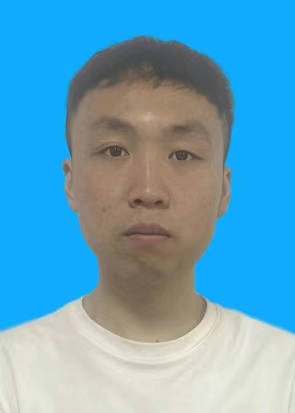
\includegraphics[width=1in,height=1.25in,clip,keepaspectratio]{./fig/slef.jpg}}]{Jiahao Xiang}
%   is pursuing a Master's degree in Electronic Information at Hengyang Normal University, China. His research focuses on cryptographic engineering and efficient implementations of block ciphers on resource-constrained devices. Publications include works on lightweight cryptography optimization and contributions to open-source cryptographic projects.
% \end{IEEEbiography}

% \begin{IEEEbiography}[{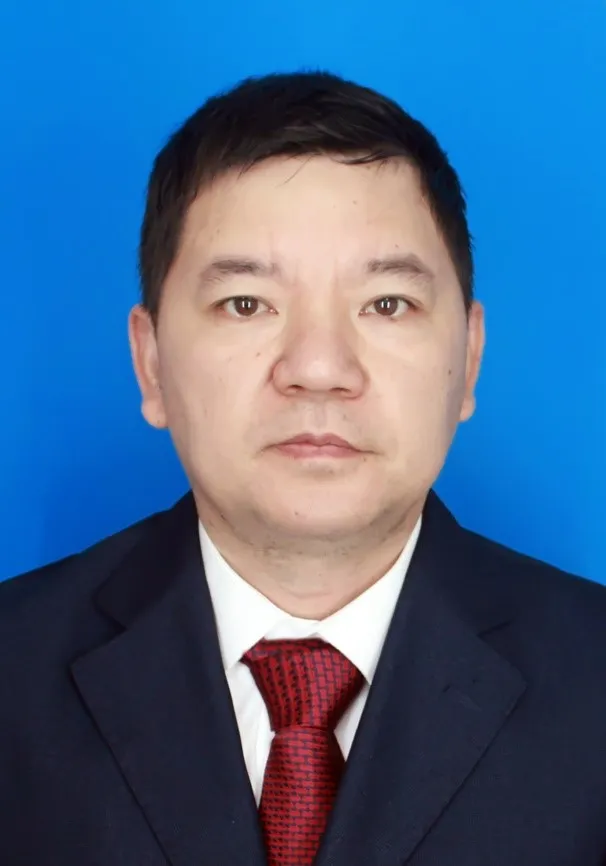
\includegraphics[width=1in,height=1.25in,clip,keepaspectratio]{./fig/boss.png}}]{Lang Li}
%   received his Ph.D. and Master's degrees in computer science from Hunan University, Changsha, China, in 2010 and 2006, respectively, and earned his B.S. degree in circuits and systems from Hunan Normal University in 1996. Since 2011, he has been working as a professor in the College of Computer Science and Technology at the Hengyang Normal University, Hengyang, China. He has research interests in embedded system and information security.
% \end{IEEEbiography}

% \vspace{11pt}

% \bf{If you will not include a photo:}\vspace{-33pt}
% \begin{IEEEbiographynophoto}{Jiahao Xiang}
% is pursuing a Master's degree in Electronic Information at Hengyang Normal University, China. His research focuses on cryptographic engineering and efficient implementations of block ciphers on resource-constrained devices. Publications include works on lightweight cryptography optimization and contributions to open-source cryptographic projects.
% \end{IEEEbiographynophoto}

% \begin{IEEEbiographynophoto}{Lang Li}
%  received his Ph.D. and Master's degrees in computer science from Hunan University, Changsha, China, in 2010 and 2006, respectively, and earned his B.S. degree in circuits and systems from Hunan Normal University in 1996. Since 2011, he has been working as a professor in the College of Computer Science and Technology at the Hengyang Normal University, Hengyang, China. He has research interests in embedded system and information security.
% \end{IEEEbiographynophoto}

\vfill

\end{document}
